
\graphicspath{{members/kh/Pictures/}}

\subsection{Leave Properties}
\input{members/kh/authors}
To achieve more realistic leaves, the simulation receives information from the modeler which analyses the structure of the different parts of the tomato plant. Since the estimation and measurements mainly focus on the leaves, the first structure analysis also just takes the leaves into account.
In the following paragraphs the leaf structure will be analyzed. First it is only looked at three structural aspects. If this approach is not meaningful after designing there are more parts that need to be analyzed later on.

\subsubsection*{Color}
The green color of a leaf comes from clorophyll. It a class of natural coloring which is produced by different organisms. 
The absorption spectrum of clorophyll is shown in Figure \ref{clorophyll}. It is shown that all wavelength accept 500nm to 600nm is being absorbed. The green color is a sign for a well functioning  photosythesis. This leads to the conclusion of a good growth and a healthy plant. Therefore healthy plants appear in a green color.

\begin{figure}[h]
	\centering
	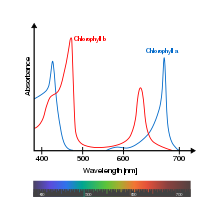
\includegraphics[width=0.4\textwidth]{wavelength.png}
	\caption{PBR Material}
	\label{clorophyll}
\end{figure}

\subsubsection*{Specularity}
Every plant has its own manner of protection. One of these manners is having special layers on the leaves. The outer layer is usually covered with different materials like cutin and natural wax which mostly contain  alcohol, alkaline and fatty acid. The Wax itself provides a certain specularity of the leaf. This specularity needs to be simulated, because there might appear some specularity effects which might change the appearance of an object that usually has a fix color. For example if light falls directly on the leaf there might appear a bright white spot. This will later on not be seen as a leaf in the total leaf area that is mesaured, because the color differs from the green that is detected. Cases like these need to b simulated to get reliable data.

\subsubsection*{Roughness \& 3D-Settings}
The stucture of the leaves might have an impact on the viewable color aswell. A leaf as we know it, is not a 2d surface, but more a three dimensional object with a certain structure. A leaf contains three major aspects that let it appear in a more threedimensional way. The first two are the leaf stem and the veins forking from it. The thrid is the microstructural setting. 
Editing the microstructural settings will be discussed in the next section. Getting a more realistic three-dimenstional object it is necessary to work with textures (\ref{textures}).

\subsection{Color- and Materialchange in Blender}
\input{members/kh/authors}

In this part we will look at the color and material change inside of Blender. As described in the section before, the plants from Plant-Studio have already been inserted and have the correct positioning. We decided to insert 10 plant randomly chosen from the 42 plants we generated before. The generated plants have a big number of leaves and fruits so we can reduce them afterwards, to have a more variant simulation. \newline
All plants together have a mean of 211 leaves and 101 fruits.
To get a more realistic and reliable model of the plants we change the color and the material of the plants. This is necessary because the leaf area algorithm needs reliable data to work with. It's easy to understand, that an object can differ in the appearence when the light falls on it from different angles. Therefore we need material properties that are similar to the properties of of real leafs and fruits.
Blender gives many options to change the properties of a material. In the following we will discuss the properties: color(appearence), metallic, emission, roughness , reflectiveness and normals. These facets are part of the pbr-library in Blender(Figure \ref{pbr}).
The changes made in this section will mainly focus on the topside of the leaf(the side that faces the sun). This is based on the fact, that the leafarea is calculated by taking a snapshot from the top of the plant. The bottom-side will be irrelevant and will be neglected in the simulation.

\subsubsection*{Blender properties}
\begin{figure}[h]
	\centering
	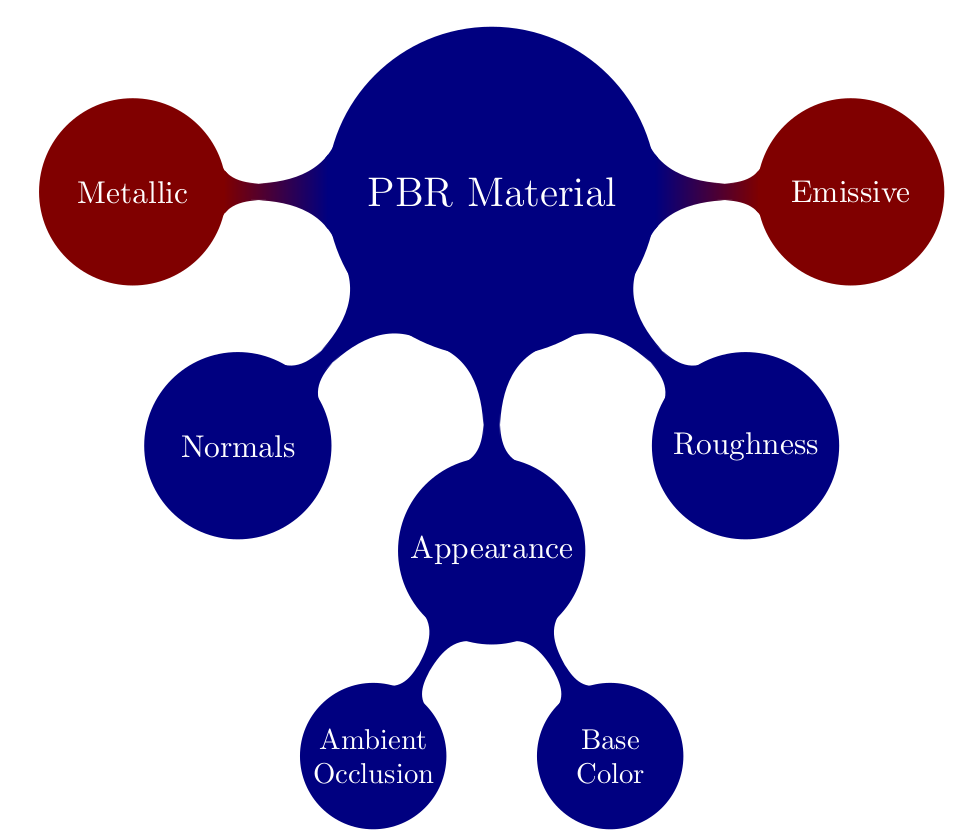
\includegraphics[width=0.6\textwidth]{blender_properties.png}
	\caption{PBR Material}
	\label{pbr}
\end{figure}
\textbf{Appearance}\\
This property can be splitted in two components. The color and the ambient occlusion. The color modifies the RGB-Values of an Object. The ambient occlusion simulates shadows between different objects, even if there is no light source in the scenery. In the simulation of the leaves and the tomatoes, the focus will mainly be on the color.\\

\textbf{Roughness}\\
The roughness is a property that is realized by a gray scale. The micro-surface of the material changes to a slightly rougher structure and this changes the looks and reflectionproperties when it comes to shading and rendering. \newline

\textbf{Metallic}\\
The option metallic is a binary map that specifies the metallic properties of a material. It is either metallic or dielectrit. It is made visible by a certain absorbtion of a material.\\


\textbf{Emission} \\
The emission describes the light a material will emit. So the material itself will become a light source and may shine. This is often used to give the scenery different illuminations. It is realized by a gray scale map that specifies the light radiation of a material, mostly to show heat or illumination.\\


\textbf{Normals} \\
A normal describes the direction an object points to. It is usually an orthogonal vector on a surface which leads to the side which shall be visible to the camera. It is important for shading, lighting  and the visibility of the surface itself.\\

\subsection{Materialchange: practical approach}
\input{members/kh/authors}

Since the leaves are already imported into blender, it is only necessary to take certain objects and color these in another color. As described before this task is approached by adding a new material to an object. In the following paragraphs the Pythoncode will be described. \newline
Coloring the leaves is performed in three steps.

\subsubsection*{Selecting Objects}
To select objects in blender a scenery has to be picked first. The scenery contains the objects that need to be edited later on. The leaves are easiely picked by looping over all elements inside the scenery. All Elements with the suffix ''Leaf'' are added to an array so they can be accessed later.
\lstset{language=Python, frame=single}
\begin{lstlisting}
# defining scenery
scene = bpy.context.scene


# fetching Leaves
leafs = [obj for obj in scene.objects
if fnmatch.fnmatchcase(obj.name, "*Leaf")]
\end{lstlisting}

\subsubsection*{Creating Material}
Since all leaves have been detected, a new material needs to be established. As described in the previous section the color, metallic, specularity and roughness of the material will be edited, so the leaf gets the structure as described.
\lstset{language=Python, frame=single}
\begin{lstlisting}
# defining a new material with name "brown"
mat_brown = bpy.data.materials.new("brown")


# setting the Properties of the material
mat_brown.diffuse_color = (0.091, 0.014, 0, 8)
mat_brown.metallic = (0.65)
mat_brown.specular_intensity = (0.5)
mat_brown.roughness = (0.55)
\end{lstlisting}

\subsubsection*{Applying Material}
To apply the material to the leaves the existing material needs to be deleted first, otherwise Blender would not set the new material as a first priority to the object. After this the material can be applied to the object. This will be performed in a loop over all elements inside the array with all leaves.

\lstset{language=Python, frame=single}
\begin{lstlisting}
#getting number of leaves
leafs_count = len(leafs)

for i in range(0, leafs_count, 1):
mesh = leafs[i]

#deleting all existing meterials
mesh.data.materials.clear()

#applying new material
mesh.data.materials.append(mat_brown)
\end{lstlisting}


\begin{figure}[h]
\centering
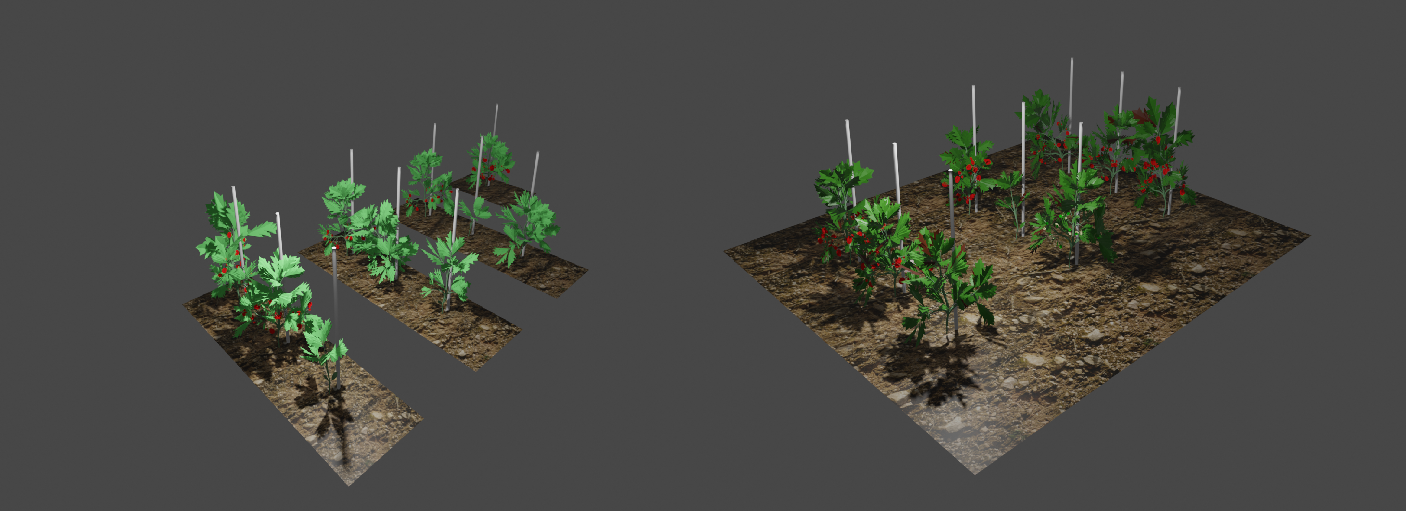
\includegraphics[width=1\textwidth]{coloring.png}
\caption{Coloring}
\label{coloring}
\end{figure}


\subsection{Removing Objects}
\input{members/kh/authors}

To approach a high variability the pregenerated plants also need to have the number of leaves and fruits reduced.
In the following it is described how the practical Aspect of removing leaves and fruits is done in Blender.
As an example it is shown how all leaves on a plant are deleted. \newline
First all leaves need to be detected and stored inside of an array. Then every element of the Array is accessed and deleted from the scenery.
\lstset{language=Python, frame=single}
\begin{lstlisting}
#fetching all leaves
leafs = [obj for obj in col.objects
if fnmatch.fnmatchcase(obj.name, "*Leaf*")]

#delete all objects inside of the Array
bpy.ops.object.delete({"selected_objects": leafs})
\end{lstlisting}
To get the same result for the fruits, the keyword ''fruit'' with wildcards surrounded needs to be accessed while fetching. A fruit in the case of the pregenerated tomatoplant is compounded by ten fruit elements to get a circular structure. To delete a whole fruit it is necessary to delete ten fruit elements. Since all elements of a fruit lay right next to each other inside the array it is easy to just loop over all fruits and delete always ten elements at a time to remove a whole fruit.
\newline
The removal of objects is shown in Figure \ref{order}.

\begin{figure}[h]
\centering
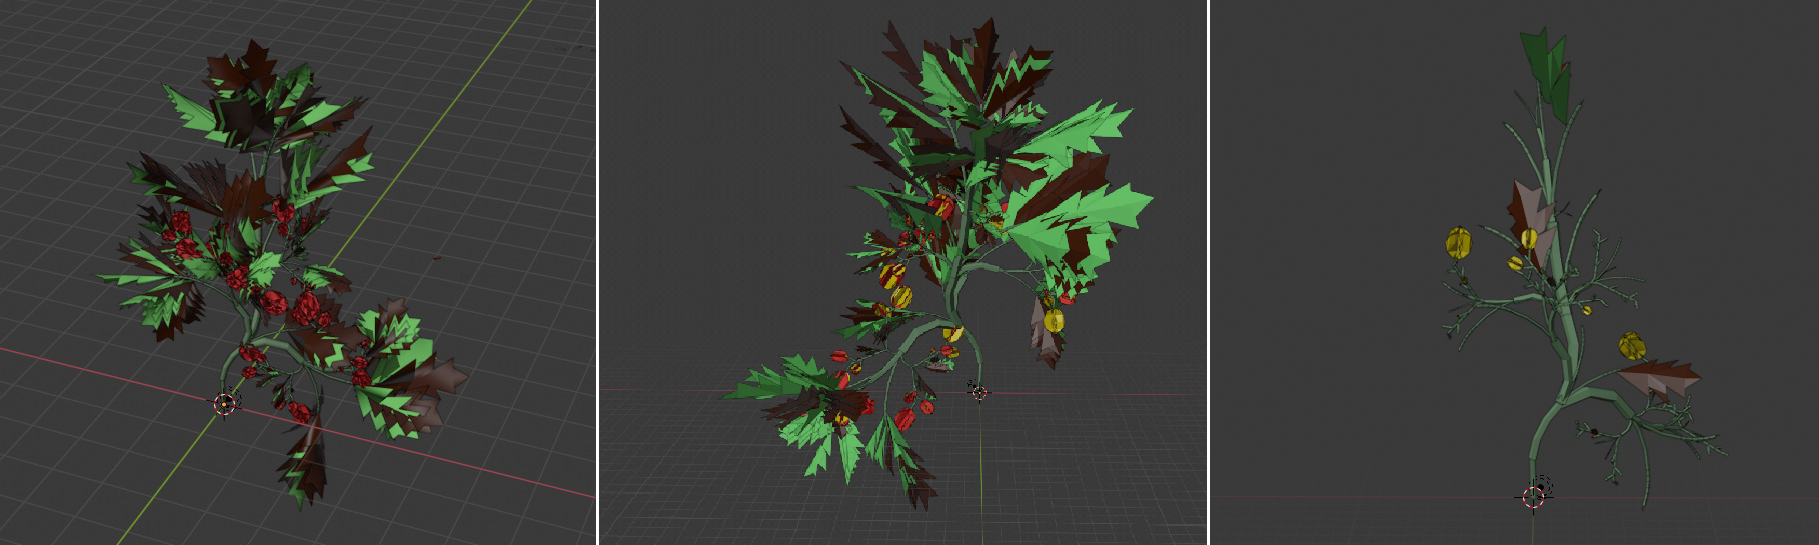
\includegraphics[width=1\textwidth]{examples.png}
\caption{Objectremoval}
\label{order}
\end{figure}


\subsection{Textures in Blender}
\label{textures}
\input{members/kh/authors}

The following section is just a small outlook. The practical implementation like applying textures or chosing the correct tools in Blender will no be discussed on this point.\newline
As already mensioned before the system needs reliable data to work with, so it is the task of the simulation to get the plants to look as realistic as possible. Real leaves have spots that reflect the light and shading that lets the collor appear differently. To apply these settings it will be necessarry to work with a texture based approach to get the leaves look better in future simulation. 
To get these textures we basically need a picture or an already existing texture. There are a few requires Stepts to apply a texture to an object in Blender, so all gaps, shades, lightings, reflections and bumps are as realistic as possible.
Overall there are a few textures needed wich can all be excluded from an already existing picture.
In the following paragraphs the textures are described an can be seen in figure \ref{textures} :

\subsubsection*{Diffuse Texture}
The diffuse texture is the original bitmap. This picture is the root where all the followig textures are generated from. This picture has to contain all information that should be added to the object inside of Blener.
\subsubsection*{Normal Texture}
The normal texture is a bumpmap. It shows small bumps and roughnesses in the structure of the object. It adds more detail to the shading, without increasing the number of polygons the object is made of. 
\subsubsection*{Specularity Texture}
The specularity texture tells the program which part of the object are glossy and which are black. The object can be reflective like metal, ceramic or plastic. It is usually a greyscale map where the black and white parts of the map highlight specularity of a pixel.
\subsubsection*{Occlusion Texture}
The occlusionmap adds more detail to the object. Is stores information about depth and shadows inside of an object. May Objects already have a more rough structure and more depth than a picture printed on an object can show.
\subsubsection*{Displacement Texture}
The displacementtexture stores the 3D information of an image. A surface is usually not 2D and in the case of a leaf it is certain that it has a structure defined my the stam and the veins goin out of it as describes by the modeler. To have these parts stick out more, the displacementmap adds the 3D details to an object.
\begin{figure}[h]
	\centering
	\includegraphics[width=1\textwidth]{textures.png}
	\caption{Diffuse/Normal/Specularity/Occlusion/Displacement}
	\label{textures}
\end{figure}
